\documentclass[12pt]{memoir}
\usepackage[backend=bibtex,style=numeric]{biblatex}
\usepackage[pdftex]{graphicx}
\usepackage{style}

\addbibresource{references}

\title{}
\author{Andrew Head}

\begin{document}

\definition{Title}{Supporting Systematic Code Inspection During Opportunistic Programming}

\definition{Author}{Andrew Head, PhD Student, UC Berkeley}

Clarke~\cite{clarke_what_2007} introduced the persona of an \emph{opportunistic developer} to describe a software developer who writes code in an ``exploratory fashion'' and develops a ``sufficient understanding of a technology to understand how it can solve a business problem''.
(This contrasts with the \emph{systematic developer}, who writes code defensively and ``develops a deep understanding of a technology before using it''~\cite{clarke_what_2007}.)
In their study of exhibit designers at San Francisco's Exploratorium interactive science museum, Brandt et al.\ reported on a group who engaged in \emph{opportunistic programming} who weren't professional developers~\cite{brandt_opportunistic_2008} but were very much what might be considered as end-user programmers --- those developing code for personal rather than public use~\cite{ko_state_2011}.

Brandt et al.\ associated several habits with opportunistic programming that are counter to what we would hope for students working with code or end-users developing a better understanding of code.
Those programming opportunistically likely to incorporate functionality by copying and pasting code, often from online sources~\cite{brandt_two_2009}.
They are more likely to implement functionality from scratch for well-known libraries, instead of reusing existing systems and libraries~\cite{brandt_opportunistic_2008}.
They also practice ``code satisficing'', implementing functionality in a sub-optimal way in order to maintain flow and move on to other functionality~\cite{brandt_opportunistic_2008}.
While opportunistic programming is powerful in that it allows one to rapidly prototype and ideate and that it reduces the cycle time of editing and debugging code~\cite{brandt_opportunistic_2008}, this behavior discourages the formation of new mental models and an introduction to new tools that should be encouraged for both novice programmers and many end-user programmers.

\if 0
This involves the reuse of components found across the web into developing working code for their personally-determined purpose, in many cases ``hacking, mashing and gluing'' code from many different sources~\cite{hartmann_hacking_2008}.
Programming enrollments have increased on college campuses, and online platforms have been developed to encourage programming learning outside of the campus, often free of tuition (e.g., Khan Academy).
In addition, it has been shown that professionals such as designers may lack formal training in programming, but reuse code and examples that they find online in their work, perhaps even without understanding exactly what the code does~\cite{dorn_learning_2010}.
\fi

As opposed to physical crafts like wiring up circuits or crocheting, programming is often text-heavy, and lacks the convenient physical affordances that convey whether an error has occurred (a mis-stitching or a wire to an incorrect terminal) while also involving the use of potentially many unknown components in the forms of APIs.
For example, for our upper-division user interface design course, students may be expected to learn new APIs for notifications, message passing, connecting to Twitter, and reading values from the system sensors, all in the same piece of code, within a couple of weeks.
Reasoning about the work produced at an atomic level, in this case functions, the arguments that are provided to them, and how these connect into larger blocks of code, is costly in the moment, so programming learners may not develop a serious understanding of the primitives out of which they build their programs.
This is a serious problem: students who don't understand these components encounter substantial difficulties debugging their programs and, as a result, developing systems with complex behavior in a short time.
(Because of the ease of copy and paste, the complexity of past work incorporated is gleefully hidden away --- until it comes to time for either error correction or designing new functionality, when major obstacles are encountered.
How do we prevent these struggles from occurring in the first place through new interactions?)

This is an entirely new environment for both development as well as the learning of a craft, in the speed of reuse of past work of others, the scale of the group of practitioners who practice it, and the shallowness of knowledge about a complex craft to repeat the techniques produced by others.
This ultimately leads us to a question: In today's development paradigms where programmers reuse code snippets and programming opportunistically at high speeds, what interventions must information seeking tools and development environments provide to encourage critical engagement and understanding of code for programmers who have not yet developed or lack the scaffolding to develop discipline and workflows for seriously understanding the code they are using?  Despite a growing prevalence of opportunistic programming as a practice, current research in programming behavior, languages, search interfaces, and tools has left this question largely untouched.
(In the interest of space, only a few examples of related research are referenced here.) However, with large numbers of programmers learning the craft through online resources, this problem becomes large scale and, due to the fact that some of these programmers may some day write personal code that is shared online, crucial to solve.

In my research, I instrument today's current programming tools with components reminiscent of intelligent tutoring systems that encourage critical engagement with found code for programming learners.
Through this research, I hypothesize that interventions for programming learners increase not only programmers' conceptual understanding of the code they develop, but also enable more accurate feasibility assessments and code design in future work.
Furthermore, I develop software that embodies these interventions, assessing both the points of contact where these interventions should occur (at copy? At paste? At a timer completion?), the types of questions that can be generated.

The work that I develop falls into three areas of areas that are currently lacking in providing critical support to opportunistic programmers who lack formal process when learning about the code they use:

\begin{itemize}
\item Techniques for automatically generating instructive explanations and demonstrations of found code
\item Interfaces for critical inspection of alternatives when selecting code for reuse
\item Intelligent tutoring-based interventions in the browser and development environment that encourage critical, just-in-time engagement with reused code
\end{itemize}

I have currently made progress on the first two of these three projects.
In the first research thrust, a recent paper I recently presented at VL/HCC, named Tutorons, explored techniques for automatically processing web content, detecting and explaining cryptic programming languages in regions of code through natural languages and demonstrations of example data.
In a small user study, the system was shown to reduce the number of accesses to external documentation needed to modify online code to perform new tasks.
Towards the second thrust, I have taken preliminary efforts to developing a visual search interface for StackOverflow questions that have a multitude of answers to ask the question: what visual affordances and interactions enable the selection of the most appropriate code examples and explanations when many sources claim to solve a user's problem?  Towards the third thrust, preliminary studies have revealed a need for more critical engagement in coding to enable the development of more secure code.
My past work in intelligent tutoring games (ToneWars) provides a tangential knowledge of the techniques in effective learning interventions, although further work will be needed to adequately address this problem.

\begin{figure}%
  \centering
  \parbox{.45\textwidth}{%
    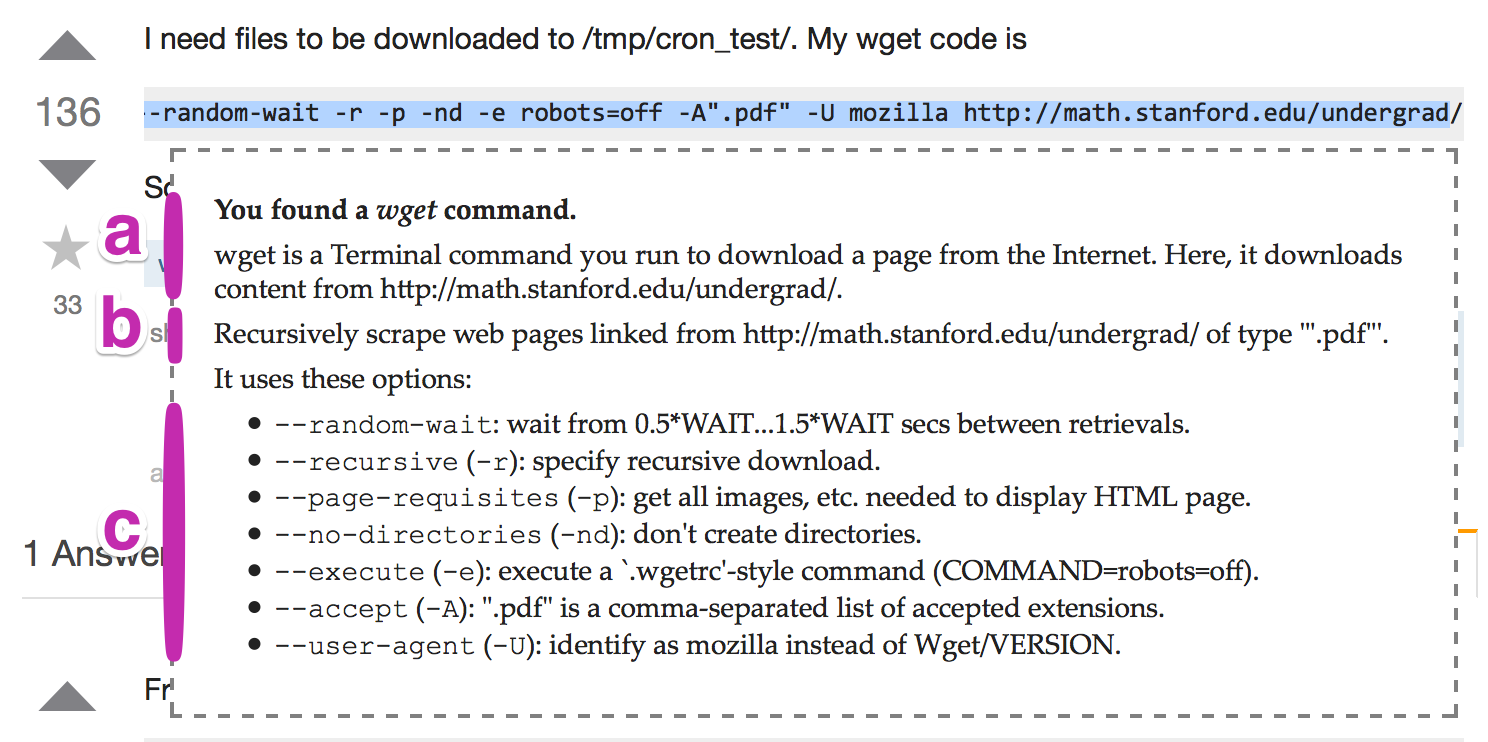
\includegraphics[width=\linewidth]{figures/tutorons_microexplanation}
    \caption{%
      A micro-explanation for a command line generated by a Tutoron with multiple levels of detail 
      (definition, high-level intent, arguments)
    }\label{fig:tutorons_microexplanation}
  }%
  \qquad
  \parbox{.45\textwidth}{%
    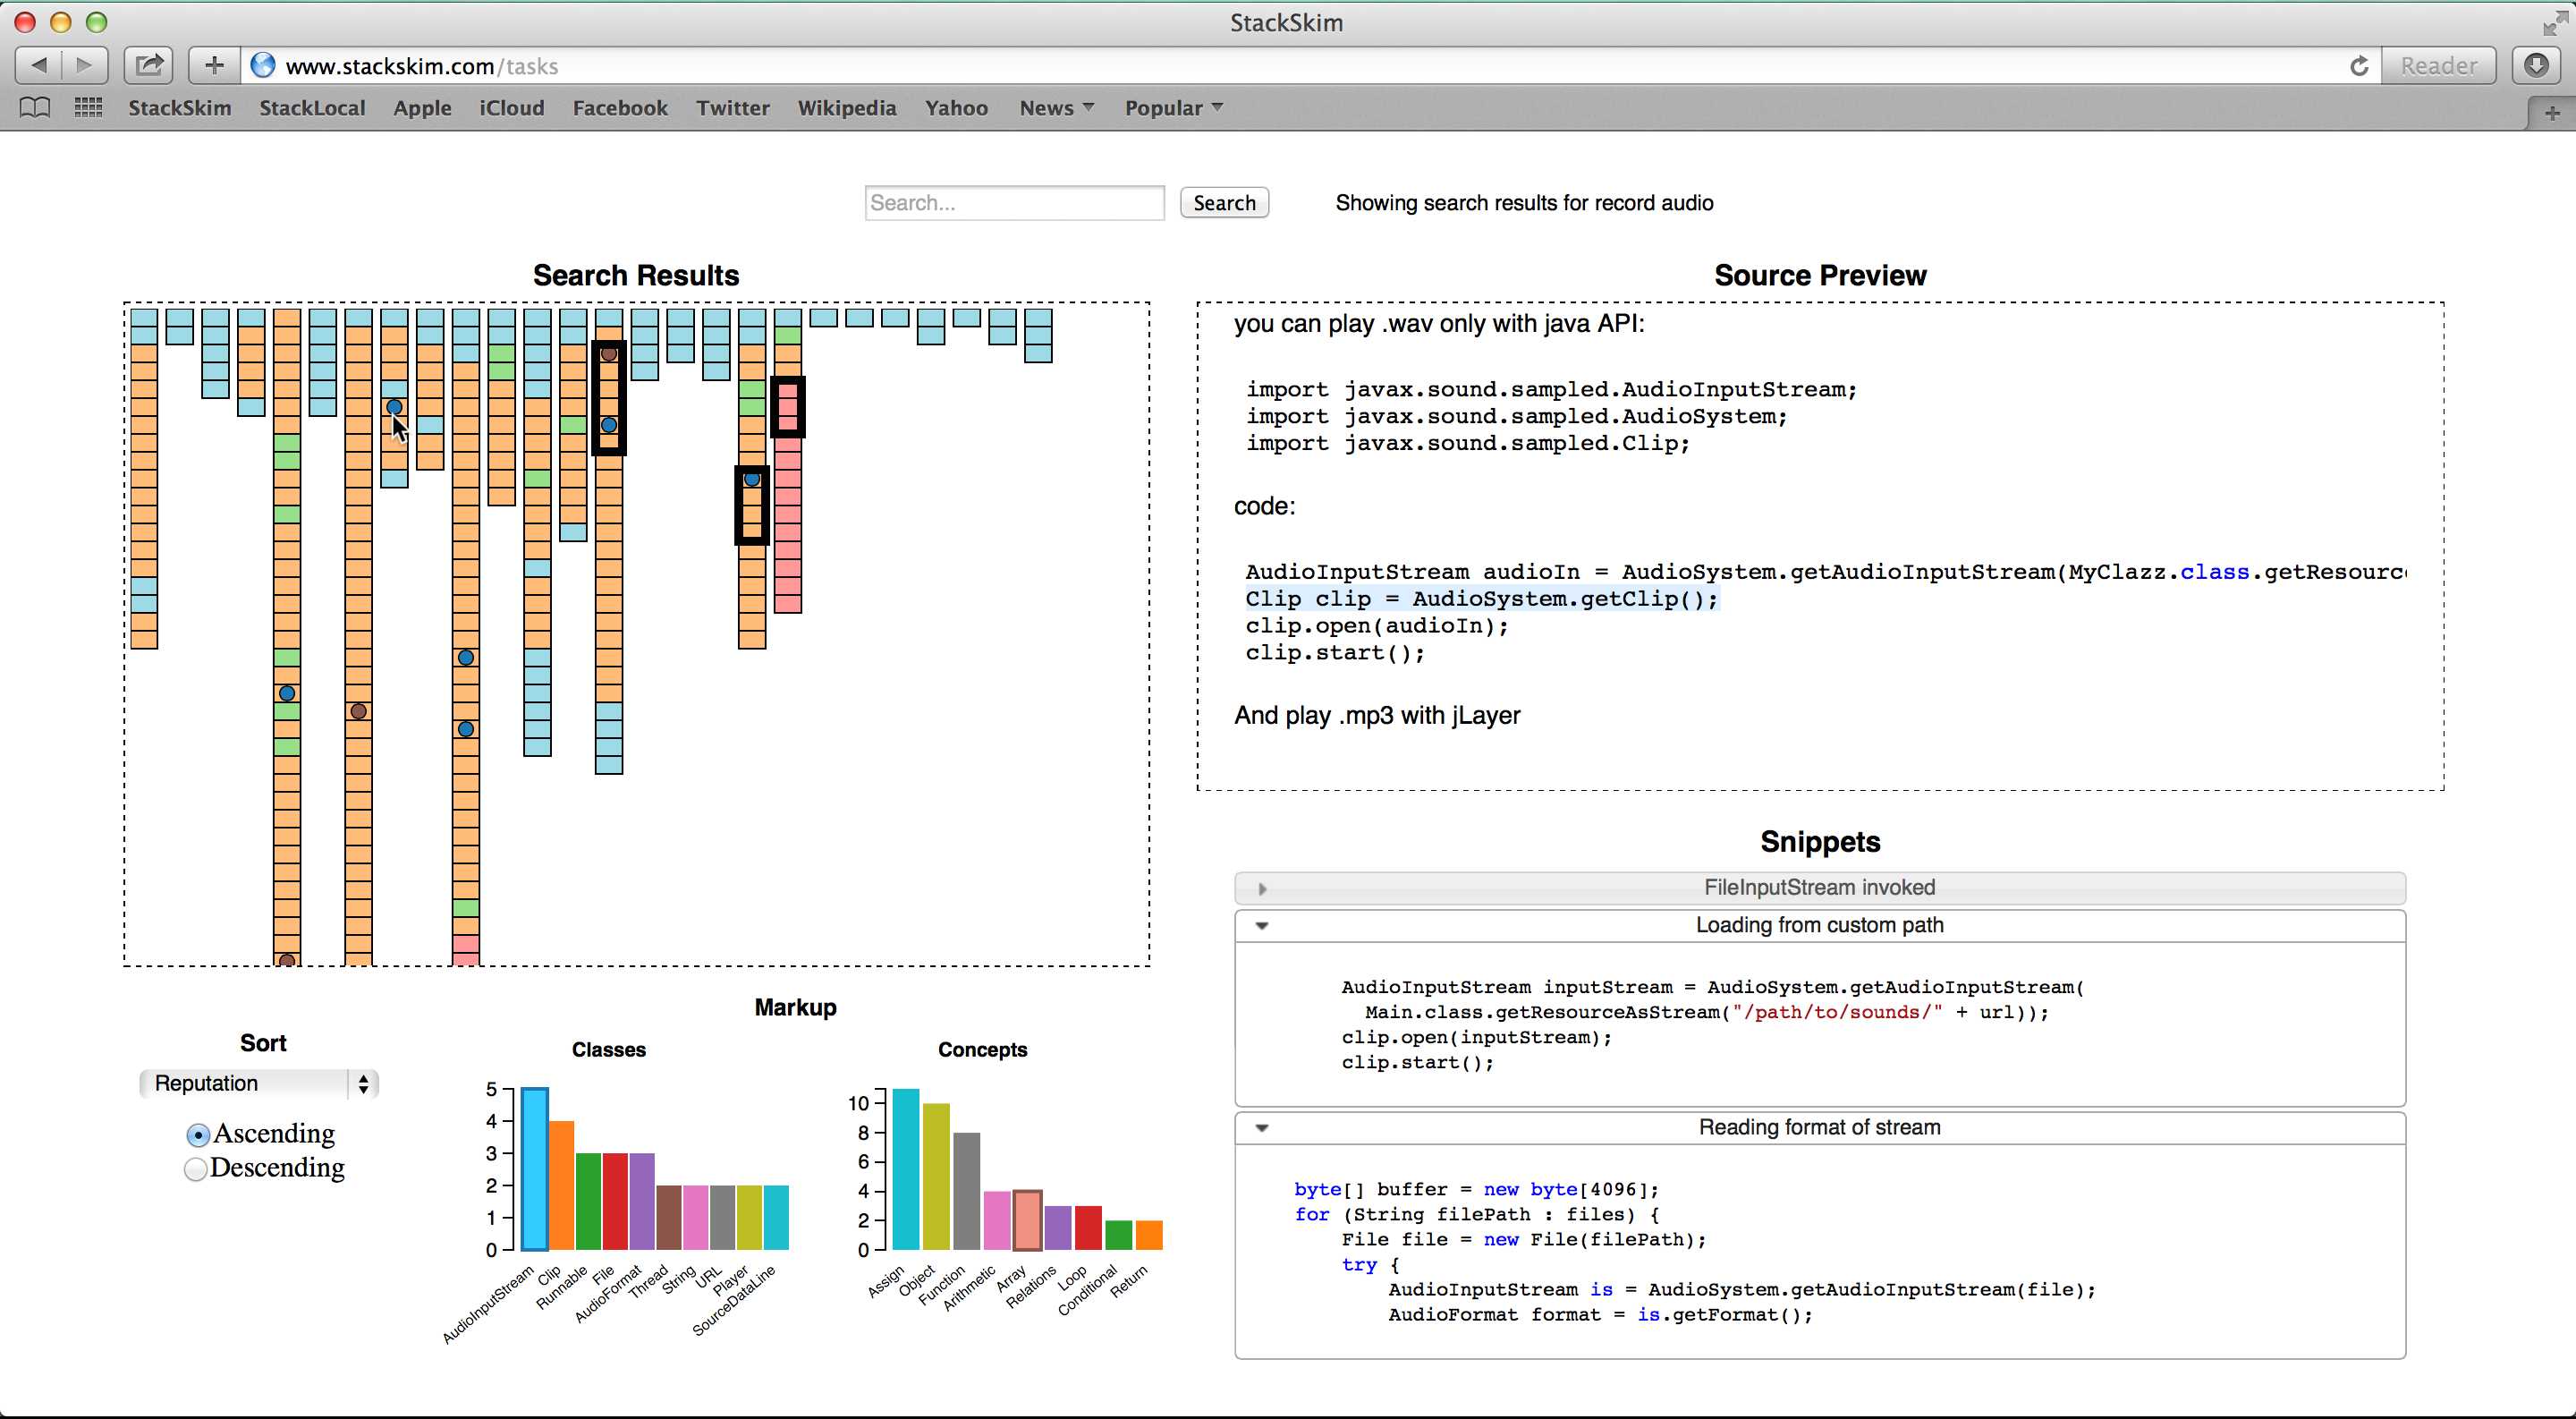
\includegraphics[width=\linewidth]{figures/stackskim_ui}
    \caption{%
      StackSkim, a visual interface for comparing and noticing trends in large collections of code examples that solve the same problem.
    }\label{fig:stackskim_ui}
  }
\end{figure}

Each of these research thrusts either has relied or will rely on the development of a software system to aid programmers in understanding code during an opportunistic programming task.
Each one also uses a mixed methods approach of observation and controlled experiments to determine how these tools indeed alter not only the task of opportunistic programming, but also programmers' behavior in selecting, understanding, and using code found online.

What comes next?  More serious development of example code, and in particular, the development of 2--3 interfaces for interventions at various levels to see what level of interventions best enable programming learners to seriously learn from the code they use when using materials found in the wild world wide web to develop without learning scaffolding or an already concrete knowledge of the tools they're using.

\section{References}
\printbibliography[heading=none]

\end{document}
